%------------------------------------------------------------------------------------------------------------------------------------------
% Analyza prostredku
%------------------------------------------------------------------------------------------------------------------------------------------
\chapter{ANALYTICKÁ ČÁST} \label{analyza}
\par Pro definici a zpracování dat musíme před samotným vývojem platformy provést průzkum aktuálních technologií zaměřujících se na vývoj webových aplikací a jejich výběr. Výběr technologií, které nám pomohou při vývoji je velice podstatný, protože nám urychlí dodání a co je důležitější, pozdější úprava bude značně jednodušší pokud zvolíme technologie, které nám pozdější vývoj usnadní.

\par Nejenom vývojovými technologiemi je potřeba se zabývat, ale také je nutné věnovat se aktuálnímu stavu trhu a tomu co uživatelé nejčastěji používají. Proto se v~této části zaměříme také průzkum trhu.

\section{Webové technologie}
\par Aktuální trend v~používání webových prohlížečů můžeme vidět na grafu \ref{browser-share}, kde jde jasně vidět že moderní prohlížeče v~podání Chrome a Firefox převládají nad čím dál méně používaným Internet Explorerem. Dále si uživatelé již uvědomují, že aktualizace prohlížeče je pro zachování zabezpečení nutností, a tak webové prohlížeče pomalu začínají pořádně fungovat s~novým standardem Javascriptu nazvaným EcmaSript 6 (známý též pod názvem ES2015 a ES6). \cite{es6}

\par Nový standard ES6 přináší mnoho vylepšení a mnoho optimalizací. Nicméně ani většina moderních prohlížečů nepodporuje tento standard na 100 \% -- například prohlížeč \textbf{Google Chrome} ve verzi 57 podporuje 97 \% nového standardu, obdobně je na tom \textbf{Edge} (verze 15 podporuje 95 \%) a \textbf{Firefox} (verze 52 zvládá 94 \%). \cite{es6-coverage}

\subsection{Webový aplikační rámec}
\par V~aktuální době se mnohým vývojářům webových aplikací ověřily takzvané webové aplikační rámce. Dříve hojně využívána knihovna \textbf{jQuery} má již mnoho nástupců jak v~podobě knihoven, tak i aplikačních rámců. Výhoda aplikačních rámců je že se stará v~podstatě o~veškerou složitou a neustále se opakující práci a nechává programátorovi volnou ruku při realizaci samotné aplikace. \cite{framework}

\par V~předešlém odstavci bylo použito dvou pojmů, jak Javascriptové knihovny, tak aplikačního webového rámce. Tyto pojmy dost často vedou k~hádkám a nedorozuměním, kdy valná většina programátorů nerozumí rozdílům mezi aplikačním rámcem a knihovnou.
\begin{itemize}
\item \textbf{Javascriptová knihovna} slouží ke konání jednoho úkolu. Vezměme si například výrobu kávy -- můžeme si postavit vodu na oheň ohřát ji, rozemlít zrnka kávy a tento prášek zalít horkou vodou. Každá jedna činnost by představovala knihovnu.
\item \textbf{Aplikační webový rámec} má na starosti veškerou práci a často zahrnuje přesně definovanou architekturu. Pokud použijeme příklad s~kávou, aplikační webový rámec by byl kávovar, do kterého nalijeme vodu a nasypeme kávová zrna. \cite{framework-vs-library}
\end{itemize}

\par Mezi aktuálně nejvíce rozšířené aplikační rámce patří ty, které podporují Single page appliacation a jsou to:
\begin{itemize}
\item \textbf{Angular.js} -- plnohodnotný aplikační rámec, který je v~aktuální době pravděpodobně nejpoužívanější.\footnote{Přesná čísla se určit nedají, nicméně více informací o~popularitě se můžete dočíst zde: \url{https://hackernoon.com/5-best-javascript-frameworks-in-2017-7a63b3870282\#.ufk9gznfd}.}. Je to strukturální webový aplikační rámec, pro dynamické webové aplikace. Jeho přední výhodou je, že se soustřeďuje na tvoření jednostránkových aplikací, takže často snižuje počet dat nutných pro načtení a pracování s~aplikací. První datum vydaní bylo v~roce 2010 a v~roce 2016 byla vydána verze 2, která umožňuje vytvářet uživatelské rozhraní jak pro webové, tak pro mobilní aplikace.
\item \textbf{React.js} -- není plnohodnotný aplikační rámec, jako \textbf{Angular.js}, nicméně je velkým hráčem na poli vývoje webových aplikací. Jeho výhodou je jeho jednoduchost (nastavení aplikace a počáteční vývoj je velice jednoduchý), nicméně nedokáže tolik věcí co plnohodnotný rámec. Samostatný ovšem není příliš vhodný, potřebuje několik rozšíření, které z~něho udělají silnějšího hráče, to ale vede k~jeho zkomplikování  a častým problémům s~nastavením.
\item \textbf{Vue.js} -- progresivní rámec pro vytváření uživatelských rozhraní. Jeho tvůrci kladli důraz na jednoduchost jeho použití a inspirovali se v~\textbf{React.js}. Výhodou oproti zmíněnému React.js je použití s~webovou stránkou, kdy se nesnaží obcházet její vykreslování, ale pracuje přímo s~html elementy. Dále je tento rámec také zaměřen na práci s~jednostránkovou aplikací, takže je výborným kompromisem mezi \textbf{Angular.js} -- který může být příliš náročný pro pochopení, a \textbf{React.js} -- který může vést ke zkomplikování při použití s~více rozšířeními.
\end{itemize}

\subsection{Silné vs. slabé typování}
\par Pro vývoj responzivních webových aplikací se používá Javascript, který je ale slabě typovaný. To znamená, že proměnná nemá předem určený pevný typ a může ho během chodu aplikace měnit. To může mít za následek chyby spojené s~očekávaným typem, který může být chybný. Takže například při očekávání čísla budeme sčítat, ale aplikace nám během jejího chodu vrátila text. Takový problém může vést až k~pádu, případně zamrznutí aplikace. Proto vznikl způsob jak přivést silné typování do slabě typovaných jazyků. Příkladem těchto technik jsou \textbf{Typescript} a \textbf{Flow}.

\paragraph{Typescript} je podmnožinou Javascriptu, to znamená, že veškeré soubory jsou přeloženy do předem vybrané verze specifikace a ty jsou poté spuštěny v~prohlížeči. Není tedy třeba nutit uživatele do používání jiného prohlížeče. Velkou výhodou je také to, že se tým okolo Typescriptu snaží co nejvíce sledovat trend vývoje Javascriptu a tak přináší mnoho novinek ještě před tím, než je začnou používat prohlížeče. Takže je možné použít velkou část nových technologií bez nutnosti psát ne zrovna příjemně čitelný kód.

\paragraph{Flow} je další způsob, jak přivést silné typování do světa Javascriptu. Oproti \textbf{Typescriptu} má výhody, že problémy s~implicitní deklarací, které mohou nastat během používání, aplikace jsou lépe vyhodnoceny a programátor je o~tomto informován již během překladu aplikace. Ale jeho nevýhodou je, že nesleduje takovou měrou nejnovější trendy a je často pozadu (někdy schválně, protože pro překlad novějších definic do staršího použití existují další nástroje -- jako například \textbf{Babel}\footnote{Více o~této technologii můžete dozvědět zde: \url{https://babeljs.io/}.}).

\subsection{Responzivní aplikační rámec}
\par Pro usnadnění používání webových aplikací na jakémkoliv zařízení vzniká aktuálně mnoho knihoven a aplikačních rámců, které mají za úkol sjednotit design napříč několika aplikacemi a také jejich responzibilitu. To znamená, že stejná aplikace se bude chovat a vypadat stejně bez ohledu na to, na jakém zařízení ji otevřeme (mobilní zařízení, tablet, počítač, televize, atd.)

\begin{itemize}
\item \textbf{Material design} -- vznikl na popud zjednodušení a zpřehlednění uživatelského rozhraní, jeho hlavním zaměřením je dotek, hlas a kliknutí. Definuje tři pravidla:
\begin{enumerate}
  \item \textbf{Material je metafora} -- chytře využívat prostor a pohyb jednotlivých elementů.
  \item \textbf{Tučné, grafické, záměrné} -- základními stavebními bloky jsou typografie, mřížka, místo, barva a použití obrázků.
  \item \textbf{Pohyb má význam} -- pokud uživatel vykoná nějakou akci design mu napoví jaká akce se stane pohybem. \cite{material}
\end{enumerate}
Příklad aplikace napsané pomocí Materialu můžeme vidět na obrázku \ref{material-fig}.

\begin{figure}[h!]
\centering
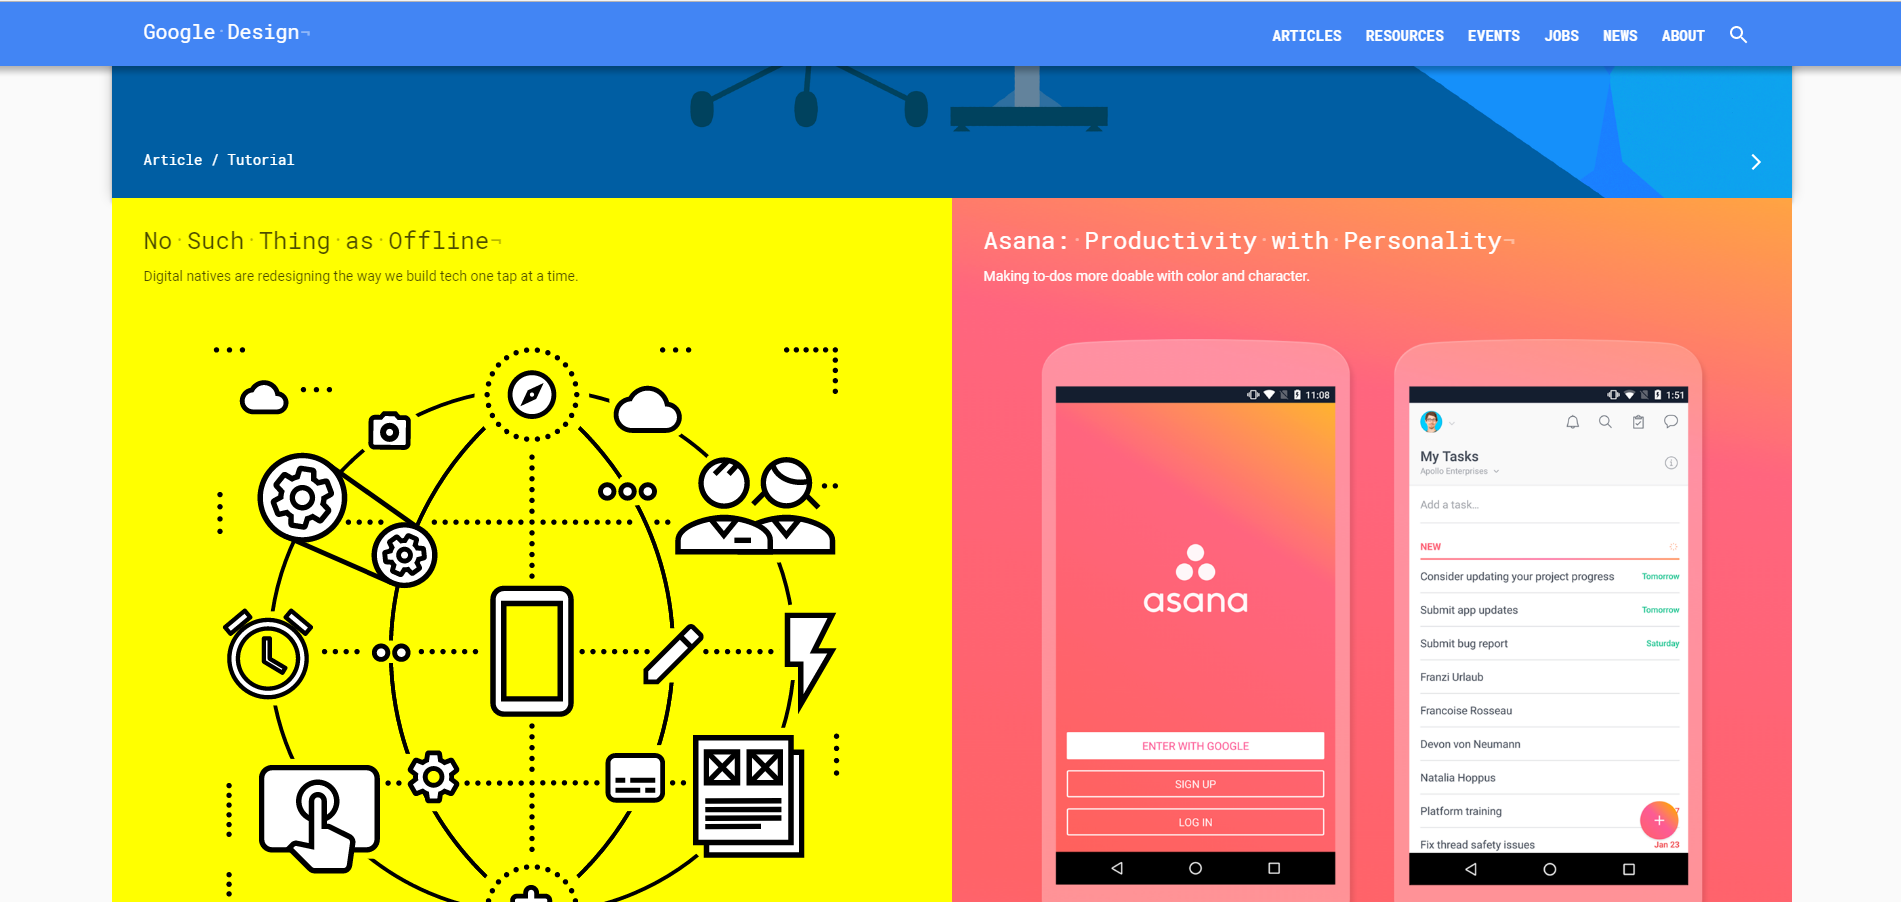
\includegraphics[max size={\textwidth}]{material}
\caption[Příklad tématu pro aplikaci napsanou technologií Material]{Příklad tématu pro aplikaci napsanou technologií Material. Zdroj: \cite{material}}
\label{material-fig}
\end{figure}

\item \textbf{Boostrap} -- jeden z~prvních responzivních rámců, který přivedl sjednocení uživatelského rozhraní napříč všemi platformami s~největším důrazem na mobilní platformy. Dost často jsou vytvořeny webové aplikace, které nerespektují různá rozlišení pro různé uživatele -- tomuto se chtěla firma stojící za aplikací Twitter vyhnout, a tak vytvořila responzivní design s~názvem Bootstrap. Nyní nabízí velké množství doplňků a rozšíření, díky kterým je z~něj dělají právem nejrozšířenější responzivní rámec. \cite{bootstrap} Příklad aplikace napsané pomocí Bootstrapu můžeme vidět na oficiálním tématu na obrázku \ref{bootstrap-fig}.

\begin{figure}[h!]
\centering
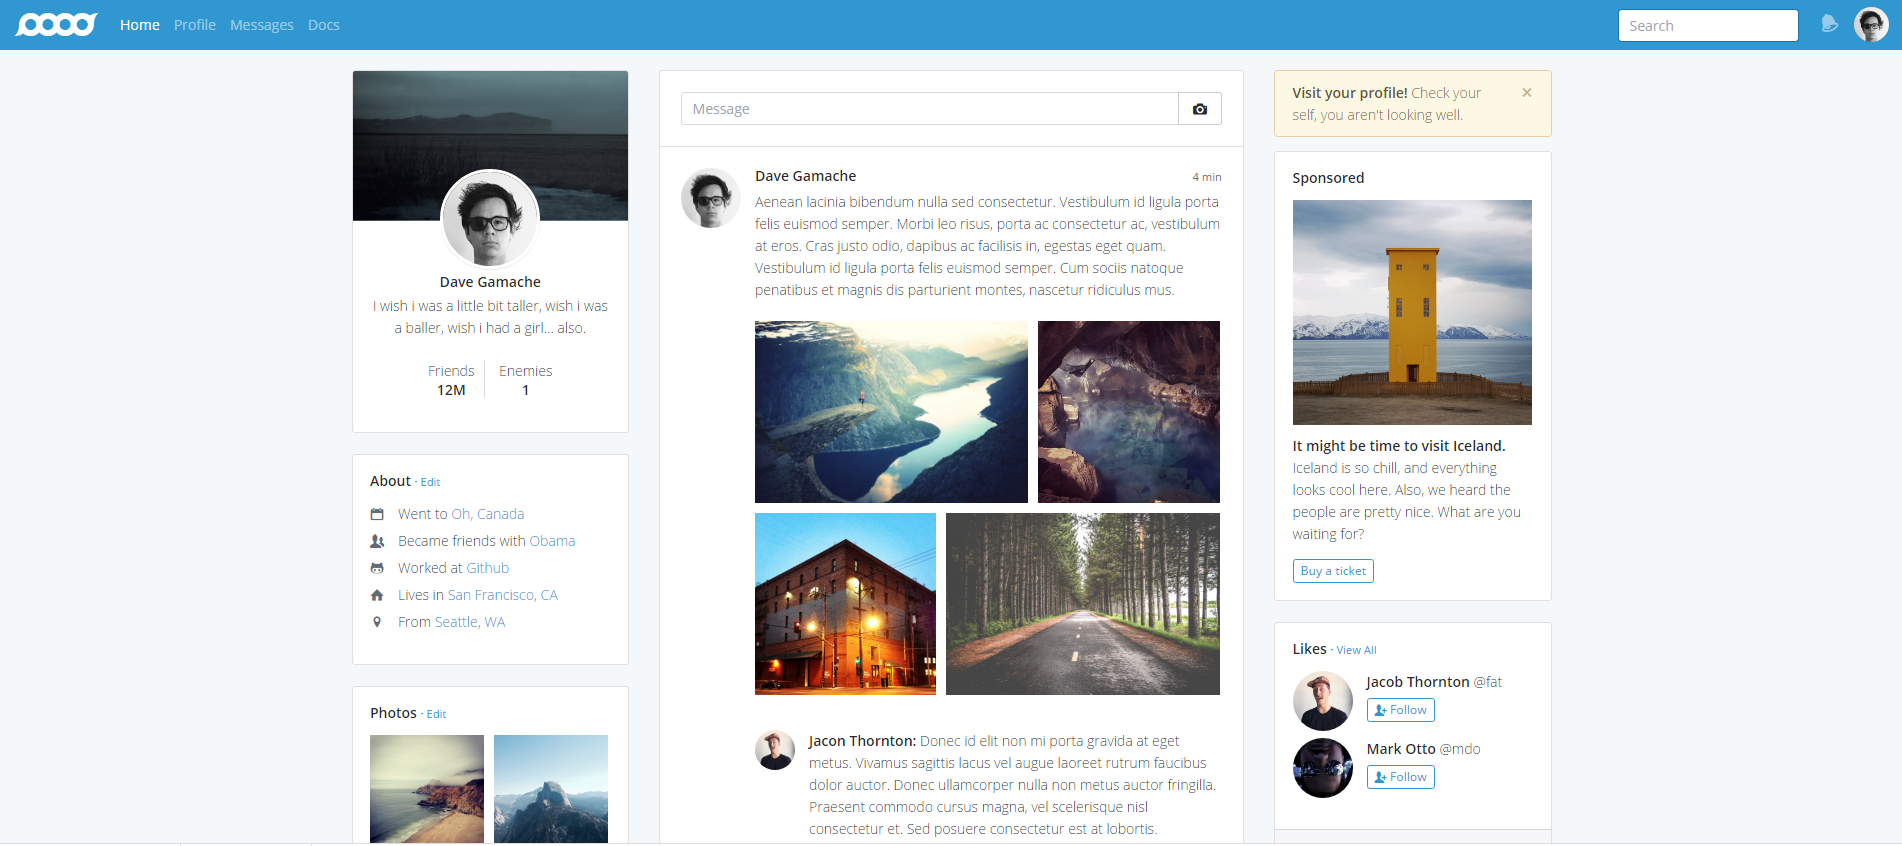
\includegraphics[max size={\textwidth}]{bootstrap}
\caption[Příklad tématu pro aplikaci napsanou technologií Bootstrap]{Příklad tématu pro aplikaci napsanou technologií Bootstrap. Zdroj: \cite{bootstrap}}
\label{bootstrap-fig}
\end{figure}
\begin{figure}[h!]
\centering
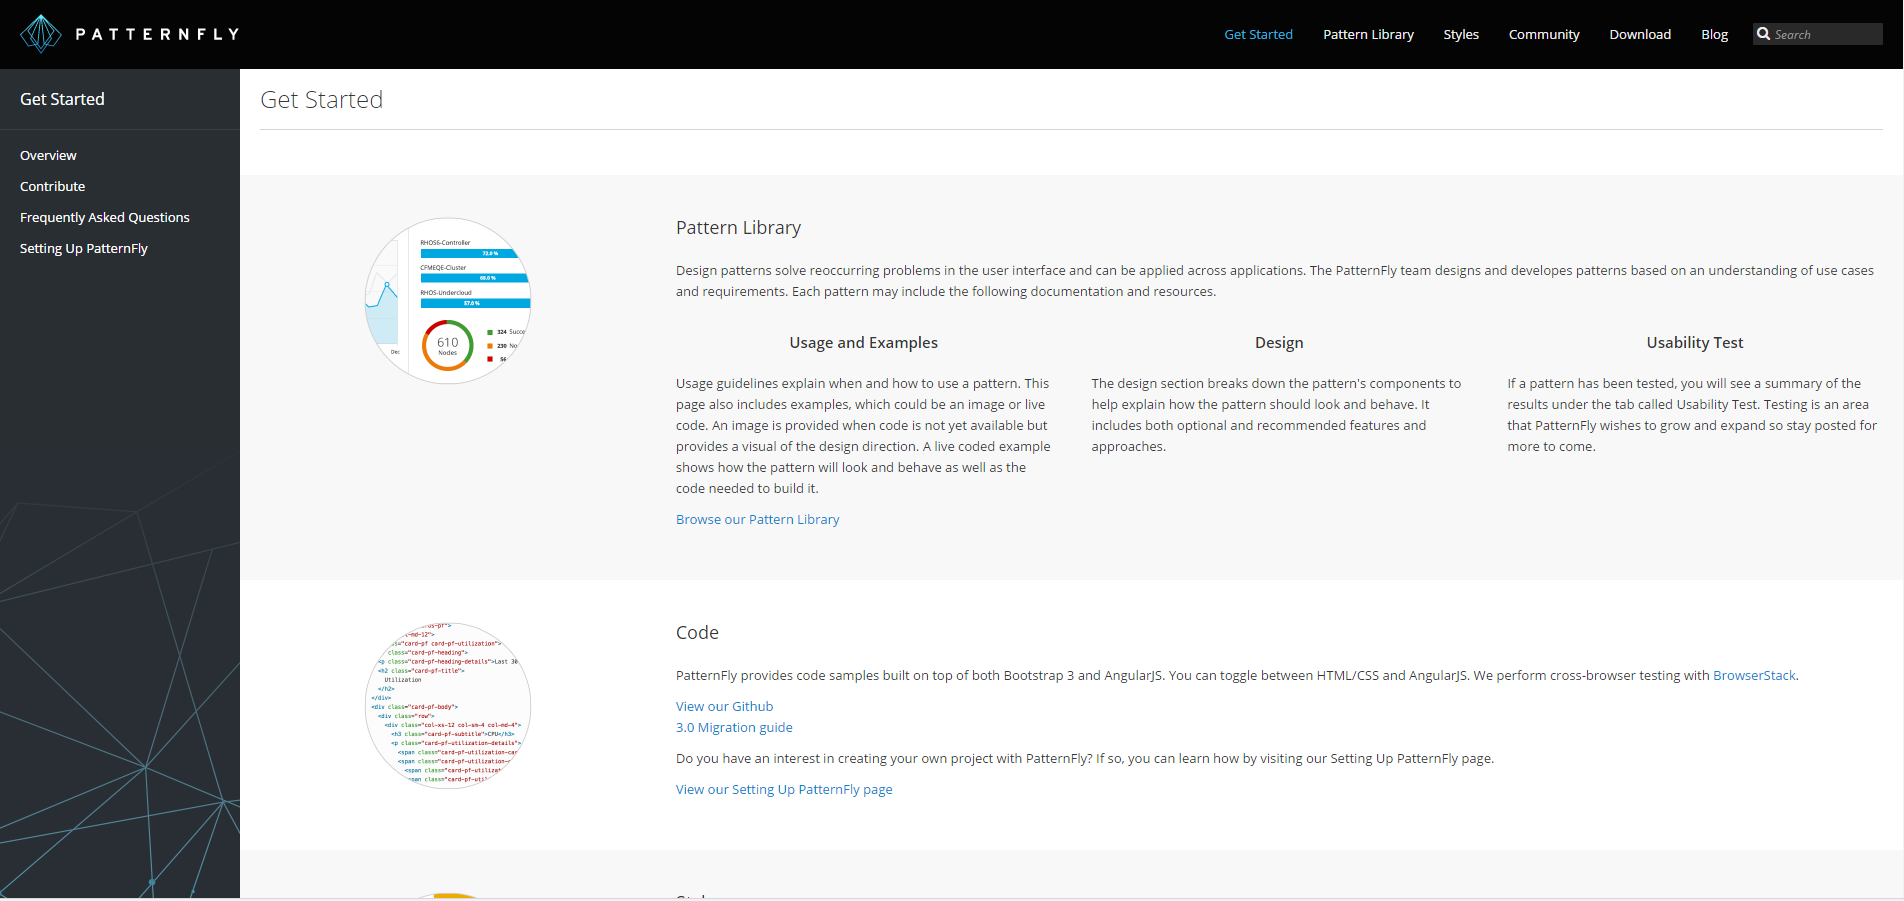
\includegraphics[max size={\textwidth}]{patternfly}
\caption[Příklad tématu pro aplikaci napsanou technologií patternfly]{Příklad tématu pro aplikaci napsanou technologií patternfly. Zdroj: \cite{patternfly}}
\label{patternfly-fig}
\end{figure}
\newpage
\item \textbf{Patternfly} -- společnost RedHat se inspiroval Bootsrapem a vytvořila vlastní responzivní rámec s~ázvem Patternfly, který dále nabízí několik widgetů pro zobrazování složitějších uživatelských dat. Jeho hlavním zaměřením je unifikovat jednotlivé aplikace ve firmě, tak aby měli stejný, ale unikátní design. Proto nabízí několik jednoduchých přístupů co a jak dělat pro dosažení co nejvíce podobného vzhledu napříč aplikacemi. \cite{patternfly} Příklad aplikace napsané pomocí Patternfly můžeme vidět na obrázku \ref{patternfly-fig}.
\end{itemize}
\clearpage
\section{Single sign-on (SSO)}
\par V~aktuální době velká část společností nabízejících větší portfolio aplikací volí takzvanou službu single sign-on, kdy uživatel nemusí pokaždé zadávat své přihlašovací údaje, ale o~jeho identifikaci se postará specializovaná služba. Většinou se stačí do této služby přihlásit jednou, a dokud nevyprší čas od posledního použití aplikace, která používá tuto službu, nebo není uživatel schválně odhlášen, nemusí se znovu přihlašovat. Jako protiklad je postaven Single sign-off, kdy při odhlášení v~jedné aplikaci je uživatel automaticky odhlášen ze všech ostatních aplikací, toto napomáhá dalšímu zabezpečení.

\subsection{Standardy získání identity}
\par V~aktuální době jsou pravděpodobně nejrozšířenější dva standardy použití SSO -- novější \textbf{OpenID Connect} a starší, ale robustnější \textbf{SAML}.

\paragraph{OpenID Connect} je v~podstatě identifikační vrstva postavená nad OAuth 2.0, poskytuje možnost identifikace uživatele a také získání základních informací. Jedná se o~modernější a v~aktuální době více používaný způsob -- převážně kvůli jeho jednoduchosti a nižšímu zatížení serveru. \cite{oidc}

\paragraph{SAML} se skládá ze dvou částí -- poskytovatele služby a poskytovatele totožnosti (tím může být například Facebook, Google, Github, atd.). Jakým způsobem je uživatel přihlášen do služby, můžeme vidět na obrázku \ref{saml2}. Nejdříve uživatel vytvoří požadavek na poskytovatele služby, ten vygeneruje SAML požadavek v~URL, aplikace přesměruje uživatele na poskytovatele totožnosti, ten ověří přihlašovací údaje, přepošle zpět na poskytovatele služby požadavek na potvrzení, dále je uživatel přesměrován na cílový požadavek, o~který si znovu požádá a server mu jej vrátí. \cite{saml}
\begin{figure}[!htp]
\centering
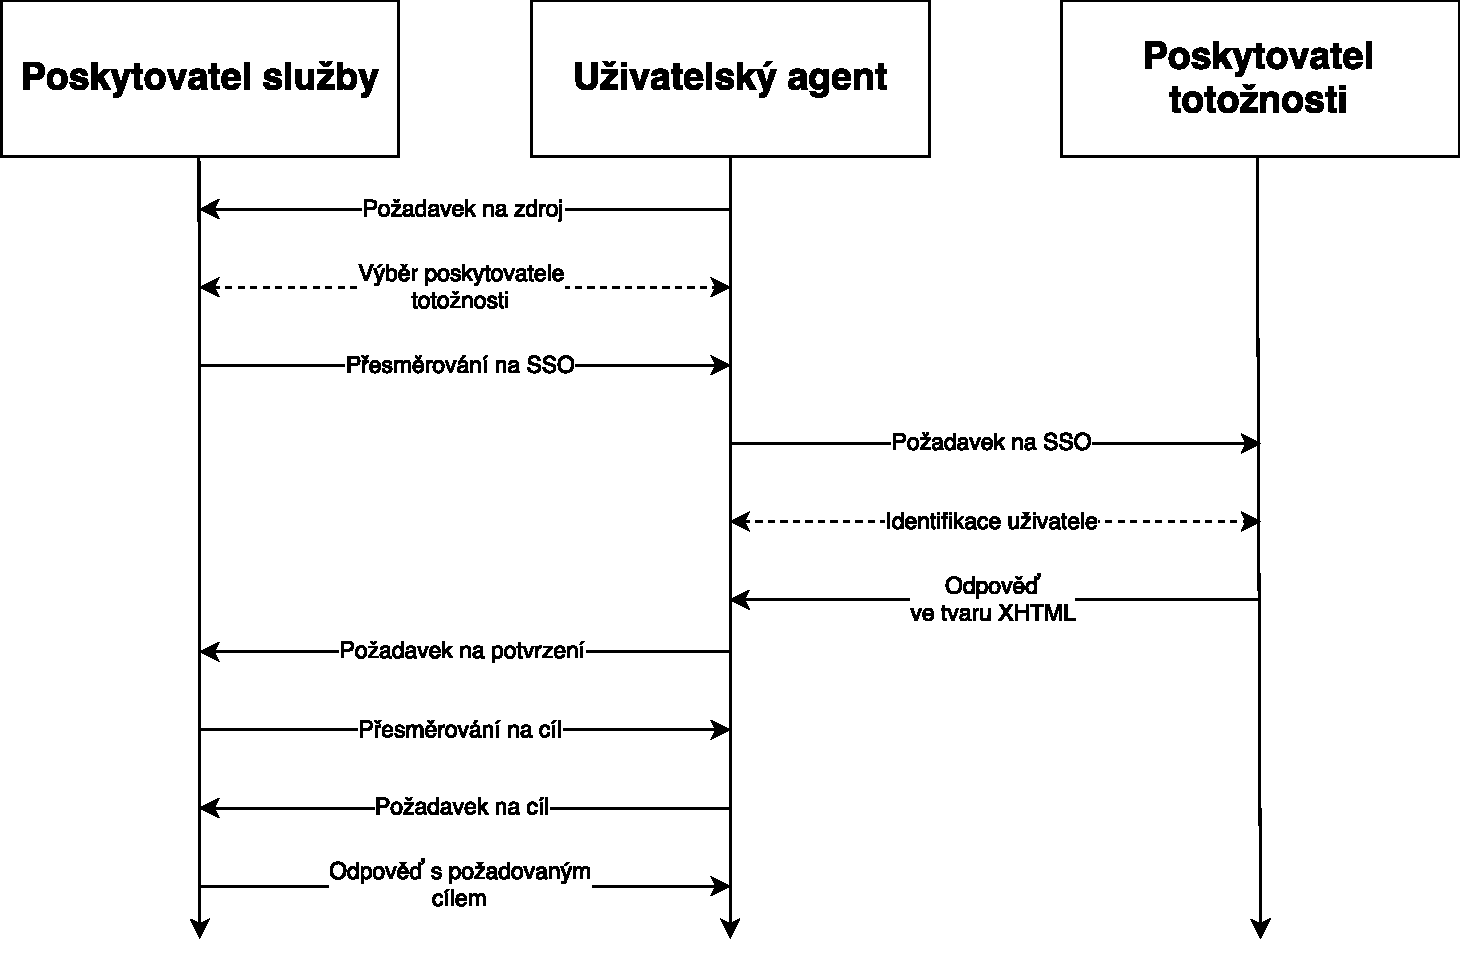
\includegraphics[max size={\textwidth}{\textheight}]{SAML2.pdf}
\caption{Předání uživatelského požadavku při použití SAML2}
\label{saml2}
\end{figure}
\newpage
\subsection{Autentikační servery} \label{auth-server}
\par Aktuální trh nabízí velké množství autentizačních serverů, které spravují uživatele a poskytují přihlášení do více aplikací. Některé jsou dokonce volně k~použití bez nutnosti zakoupit licenci -- je nutné pouze spravovat servery, na kterých takováto služba poběží. Mezi tyto servery patří například \textbf{Keycloak}, \textbf{Sterling externí autentizační server} a \textbf{Active Directory Federation Services}.

\subsubsection{Keycloak} 
\par Keycloak je open-source software řešení, které nabízí připojení i přes sociální sítě a možnost získání uživatelských účtů z~LDAP, Active Directory a nebo přímo z~databáze. Jeho velkou premisou je jednoduchost správy uživatelů, včetně definice přístupových práv pro jednotlivé části aplikace. \cite{keycloak} Jak uživatel získá JWT při použití nástroje Keycloak můžeme vidět na obrázku \ref{keycloak-jwt-fig}, kde si uživatel zažádá o~nový token, kterým se poté autorizuje u~aplikačního serveru.

\begin{figure}[htp]
\centering
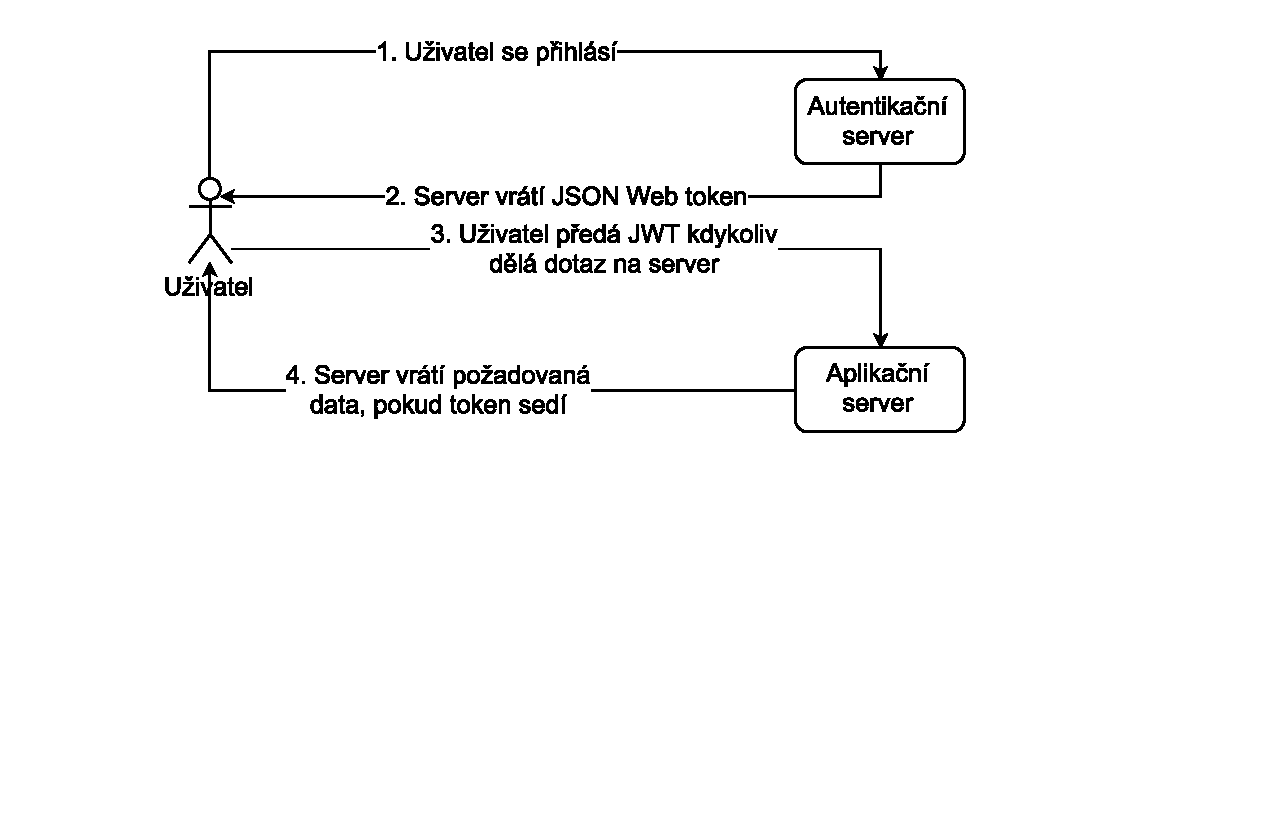
\includegraphics[max size={\textwidth}{\textheight}]{jwt.pdf}
\caption{Znázornění získání JWT z~nástroje Keycloak.}
\label{keycloak-jwt-fig}
\end{figure}
\newpage
\subsubsection{Sterling externí autentizační server}
\par Sterling externí autentizační server označuje řešení od IBM nabízející rozšířené autentizace a validace služeb pro IBM produkty. Nabízí napojení například na LDAP a možnost SSH autentizace. \cite{ibm-ster}

\subsubsection{Active Directory Federation Services}
\par Active Directory Federation Services od firmy Microsoft nabízí možnost sdílet identifikační informace napříč důvěryhodným obchodním partnerům skrze extranet. Výhodou je že se aplikace nemusí starat o~všechny uživatele, ale pouze si vyžádá od spřátelené aplikace jeho práva. \cite{ADFS}

\section{Datová analýza}
\par Pokud firma disponuje velkým množstvím dat, je vhodné nad těmito daty najít nějaké souvislosti, které jí dopomůžou k~vytváření dalšího zisku, případně pouze pro pochopení daného zákazníka, nebo skupiny zákazníků. Jestliže je těchto dat opravdu hodně, můžeme je označit za Big Data (popsáno v~\ref{big-data}), poté procesům k~získání dalších informací říkáme dolování dat (blíže popsáno v~\ref{data-mining}).

\subsection{Shluková analýza}
\par Pro bližší pochopení velkého množství dat je vhodné použít metodu shlukové analýzy, což je zjednodušený proces organizace objektů do skupin tak, aby prvky v~jedné skupině byly nějakým způsobem co nejvíce podobné. Shlukovou analýzu můžeme rozdělit do dvou skupin \textbf{nehierarchické} a \textbf{hierarchické}.

\subsubsection{Nehierarchické}
\par Nehierarchické metody mohou být tvrdé nebo jemné. Tvrdé seskupují data na základě specifické shlukové vlastnosti -- pokud patří do tohoto shluku nemůže patřit do jiného. Jemné na druhou stranu nedefinují přesnou hranici -- patří do tohoto shluku, ale má některé vlastnosti datových bodů jiných shluků. Pro dělení můžeme použít metodu K-means, která přiřadí každý bod do shluku jehož středu je nejblíže a při každém běhu algoritmu se středy shluků přepočítávají jako aritmetické průměry všech bodů. \cite{big-data-anayitics}

\subsubsection{Hierarchické}
\par Hierarchické metody můžeme použít ve dvou způsobech -- ze shora dolů a odspodu nahoru. V~prvním případě vezmeme všechny datové body a označíme je za shluk, který poté rozdělíme na další shluky, které dále dělíme. Opět můžeme využít K-means pro dělení shluků. Druhý způsob (odspodu nahoru) je nejlepší použít v~případě že máme menší vzorek dat a chceme co nejlepší shluk. \cite{big-data-anayitics}

\subsubsection{Shrnutí}
\par Při použití shlukové analýzy musíme odpovědět na dvě otázky.
\begin{enumerate}
  \item \textbf{Jaký je nejmenší počet shluků?} -- Na první otázku je jednoduché odpovědět, je to v~podstatě celý seznam datových bodů v~jednom shluku.
  \item \textbf{Jaký je největší počet shluků?} -- Odpovědí může být počet všech datových bodů.
\end{enumerate}
Proces shlukování je tedy rozdělování těchto dat do shluků větších jak jedna a menších než počet prvků, proces ukončíme v~momentě, kdy jsme spokojeni s~celkovým počtem shluků, případně velikostí těchto skupin. \cite{data-mining-practical}

\subsection{Rozhodovací stromy}
\par Algoritmus rozhodovacích stromů slouží k~získání pravidel a vztahů v~datovém souboru pomocí větvení. Díky použití stromů je tento algoritmus rychlý a výhodný pro použití s~počítačem. Složení stromu je takové, že na vrcholu je jeden uzel, kterému se říká kořen, ze kterého vede několik hran spojujících vnitřní uzly, které mají opět několik hran propojujících další uzly. Každý uzel musí mít právě jednoho předka (ne více ani méně), kromě kořenového uzlu, který nemá žádného předka. Výhodou je jednoduchost, efektivnost a možnost použít i pro velký objem dat. Na druhou stranu pokud nám budou některá data chybět, nebo budeme mít spojitá data rozhodovací stromy budou mít problémy. \cite{data-mining-principles} Při výběru vlastnosti, která je nejvíce odlišná od ostatních příkladů v~ostatních třídách se požívá takzvané entropie -- její výpočet lze vidět na \ref{entropie}, kde \(p_t\) je pravděpodobnost výskytu třídy \(t\) a \(t\) je počet tříd.
\begin{equationcap}[!htp]
\centering
\begin{equation} \label{entropie}
E(S) = - \sum_{t=1}^{T}(p_t log_2 p_t)
\end{equation}
\caption[Vzorec pro výpočet entropie v~rozhodovacích stromech]{Vzorec pro výpočet entropie v~rozhodovacích stromech. Zdroj: \cite{data-mining-principles}}
\end{equationcap}

\par Pro vytvoření stromu se vezme tabulka hodnot a pro každý atribut se vypočítá jeho entropie -- ta znázorňuje homogenitu prvku. Pokud je prvek naprosto homogenní (nacházející se ve všech atributech), jeho entropie je 0, naopak pokud je prvek naprosto heterogenní (nachází se pouze v~jednom atributu), jeho entropie je 1. Při prvotním vytvoření rozhodovacího stromu je tedy potřeba mít co nejlepší trénovací data, nicméně velké množství dat může mít za následek příliš složitý strom, který je opět nepoužitelný (proto je potřeba dbát na vhodnou velikost učebních dat). Pokud nám vznikne složitý a ne příliš efektivní rozhodovací strom, je vhodné použít takzvané prořezávání, kdy odstraníme nadbytečné podstromy (velice vhodné v~případě, že jsme použili velký vzorek dat pro vytvoření stromu). \cite{data-mining}

\par Příklad algoritmu, který se používá pro vytváření rozhodovacích stromů je takzvaný ID3. Ten je založen na booleovských hodnotách, používá hladové vyhledávání v~prostoru a strom je vytvářen odshora dolů. Vstupní parametry tohoto algoritmu jsou:
\begin{itemize}
\item \textbf{příklady} -- data, na kterých je rozhodovací strom vytrénován.
\item \textbf{atributy} -- nad nimiž bude strom testován.
\item  \textbf{cílový atribut} -- tento atribut se bude snažit predikovat vytvořený strom. \cite{minigbook}
\end{itemize}
ID3 algoritmus byl několikrát vylepšen a upraven pro použití za různých podmínek jako například C4.5 (vhodné při chybějících, nebo spojitých datech), C5 (vylepšený C4.5), pro vytvoření binárních rozhodovacích stromů je například vhodné použít klasifikační a regresní stromy (CART), případně pro práci s~opravdu velkým množstvím dat je možné použít algoritmus SPRINT. \cite{minigbook}

\par Na obrázku \ref{decision-tree} můžeme vidět příklad stromu, který vznikl pro rozhodování zda jít hrát badminton. Pro jeho vytvoření byl použit algoritmus ID3 s~menším vzorekem dat.
\begin{figure}[htp]
\centering
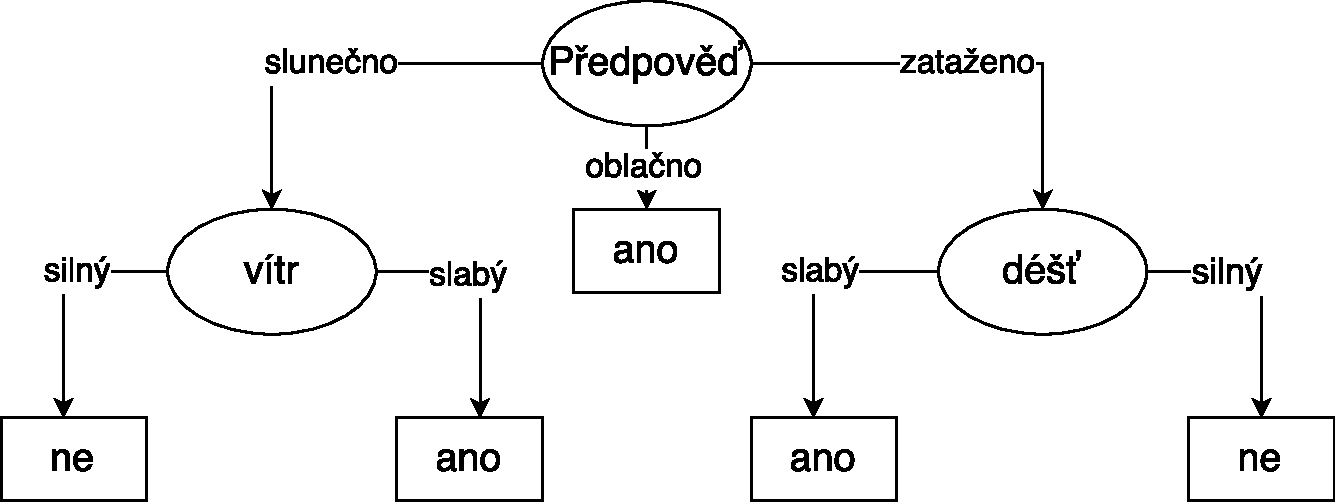
\includegraphics[max size={\textwidth}]{decision.pdf}
\caption[Příklad rozhodovacího stromu při použití algoritmu ID3]{Příklad rozhodovacího stromu při použití algoritmu ID3. Zdroj: \cite{minigbook}}
\label{decision-tree}
\end{figure}

\subsection{Dolování dat na webové aplikaci}
\par Dolování dat na webové aplikaci je získávání informací z~webových dokumentů (případně webových stránek), hyperlinků mezi webovými dokumenty a stránkami a získávání informací z~logů (serveru).

\par Na webu lze využít několik možných technik dolování:
\begin{itemize}
\item \textbf{Dolování webového obsahu} -- proces získávání informací z~webových dokumentů -- mohou to být jak samotné stránky, tak videa, zvukové stopy a obrázky. Hlavním zaměřením je však získání informací ze samotných textů na webovém dokumentu.
\item \textbf{Dolování webové struktury} -- strukturu webových stránek si lze představit jako, uzlový graf, ve kterém jsou jednotlivé uzly samotné stránky a hrany spojující tyto stránky jsou vzájemné odkazy. Lze se také dále zanořit v~jednotlivých dokumentech a ty znázornit pomocí stromové struktury\footnote{Přesný popis tohoto zápisu je znám pod zkratkou DOM (Document object model).}.
\item \textbf{Dolování webového používání} -- název pro označení technik, díky kterým lze získat další informace z~používání webových stránek. Tato data lze získat z~několika zdrojů:
\begin{enumerate}
  \item \textbf{Webový server} -- záznamy, které vygeneroval server během jeho používání (IP adresy uživatelů, navštívenou stránku a čas navštívené stránky ...).
  \item \textbf{Aplikační server} -- použití moderních aplikačních serverů dovoluje hladší vytvoření podnikových aplikací, tyto servery nadále dovolují bližší sledování uživatelských interakcí.
  \item \textbf{Data aplikací} --  získávání dalších ifnormací o~pohybu a chování uživatele na základě serverových logů (technické informace vypsané serverem s~časovým razítkem a případně navštívenou stránkou). \cite{minigbook}
\end{enumerate}
\end{itemize}

\paragraph{PageRank} slouží k~hodnocení webových stránek, které pomáhá k~tomu, aby daný web byl na vyšších příčkách ve vyhledávačíh jako Google, Seznam, Yahoo, atd. Označuje tedy metriku pro ohodnocení dokumentů a zjištění jejich kvality. Výpočet ohodnocení stránky \(p\) lze získat použitím rovnice \ref{pageRank}, kde \(n\) je počet odchozích uzlů, \(Outdegree(q)\) je počet hyperlinků na stránce q, \(d\) znamená pravděpodobnost, že uživatel zadá stránku přímo bez prokliknutí z~jiné stránky a \(1 - d\) označuje pravděpodobnost, že uživatel navštíví stránku z~prokliknutého hyperlinku. \cite{minigbook}
\begin{equationcap}[!htp]
\centering
\begin{equation} \label{pageRank}
PR(p) = d/n + (1-d) \sum_{(q,p) \in G}(\frac{PR(q)}{Outdegree(q)})
\end{equation}
\caption[Vzorec pro výpočet ohodnocení stránky]{Vzorec pro výpočet ohodnocení stránky. Zdroj: \cite{data-mining-principles}}
\end{equationcap}

\par Pro znázornění ohodnocení náhodné stránky se můžeme podívat na obrázek \ref{pageRankFig}, kde na jednu stránku ukazují tři stránky \textbf{P1}, \textbf{P2} a \textbf{P3}.
\begin{figure}[htp]
\centering
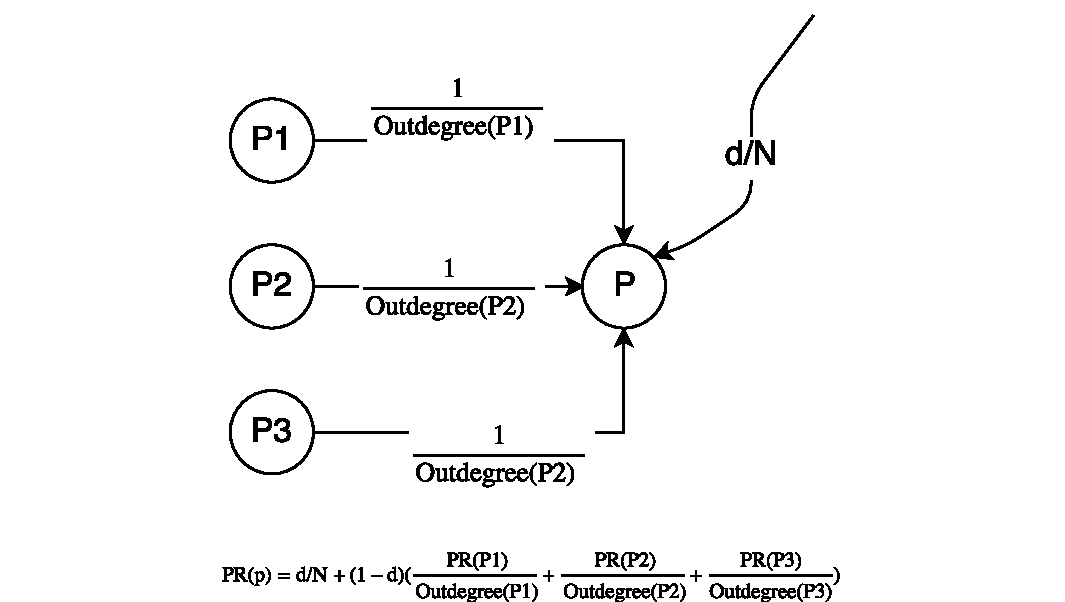
\includegraphics[max size={\textwidth}]{pagerank3.pdf}
\caption[Příklad hodnocení stránky pomocí Markovova modelu náhodné stránky]{Příklad hodnocení stránky pomocí Markovova modelu náhodné stránky. Zdroj: \cite{minigbook}}
\label{pageRankFig}
\end{figure}

\subsection{Ukládání a práce s~velkým objemem dat}
\par Při použití většiny technik na dolování dat je potřeba toto dolování spustit nad velkým množstvím dat, proto vzniklo několik technik jak na ukládání, tak na práci s~velkým objemem dat. Pro ukládání se často příliš nehodí klasická relační databáze, a proto se používají například takzvané NoSql databáze. Jednou z~technik, jak propojit několik datových uzlů, je použití takzvaných \textbf{Datové sklady} -- ty mají možnost připojit se na několik databází (bez ohledu na jejich typ) a za pomocí sofistikovaných reportingových nástrojů vytahovat z~těchto databází informace, které se dále transformují a upravují. \cite{nosql}

\par V~případě použití NoSql databáze je potřeba data nějakým způsobem provázat (indexovat), aby s~nimi šlo pracovat ve velice rychlém časovém úseku bez nutnosti při každém dotazu brát data přímo z~databáze. Mezi indexovací nástroje patří například nástroje \textbf{Solr}\footnote{Jednoduchý a otevřený indexační nástroj \url{http://lucene.apache.org/solr/}.} nebo\textbf{Elasticsearch}\footnote{Nástroj, který vyhledává a dokáže také analyzovat data \url{https://www.elastic.co/}.}

\par Pokud naopak využijeme datových skladů, můžeme pro následnou vizualizaci využít takzvané OLAP kostky, což jsou sady nástrojů pro práci s~daty (mezi tyto nástroje patří například pivoting, řezy, drill down/up atd.)

\subsection{Aplikace využívající datovou analýzu}
\par V~průběhu využívání dolování dat a využívání datové analýzy se nástroje a aplikace postupně zdokonalovaly a začínají být čím dál více uživatelsky přístupné. Firmy se snaží propojit několik takových aplikací a dát uživatelům silné nástroje pro snadné a rychlé získání dodatečných informací z~velkého množství dat. Často se objevuje možnost připojit různé zdroje dat do těchto aplikací.

\paragraph{Power BI} -- je sada obchodních analytických nástrojů od firmy Microsoft, tyto nástroje vynikají především možností připojení na velké množství datových zdrojů a také možností publikovat vytvořené reporty na webové rozhraní (na takzvaný dashboard). Pro připojení na různé datové zdroje je použit nástroj Power BI gateway, který umožňuje (mimo jiné), připojení na různé SQL databáze a analytické modely. \cite{powerbi}

\paragraph{IBM Watson Analytics} -- hlavní motto tohoto nástroje je poskytnutí silných a pokročilých analytických technik bez přílišné komplexnosti. Výhodou oproti ostatním nástrojům a aplikacím, které se věnují datové analýze, je jednoznačně možnost rychle (a bez nutnosti pokročilých technik dolování informací) získat ukryté informace v~zákaznických datech. Tohoto docílili inženýři ve firmě IBM tím, že vyvinuli velice silnou a rychlou umělou inteligenci\footnote{Více o~této umělé inteligenci pojmenované Watson se můžete dočíst zde: \url{http://www.slate.com/blogs/future_tense/2014/02/14/watson_is_real_artificial_intelligence_despite_claims_to_the_contrary.html}.}, která má za úkol hledat skrytou podstatu v~datech. \cite{watson}

\paragraph{MicroStrategy} -- platforma podporující dashboardy, interaktivní reporty a dotazování, upozornění na události a mnoho dalších technik potřebných pro vytváření strategie podniku a zjišťování informací z~dat. Tato platforma nevyužívá klasické multidimenzionální OLAP kostky, ale využívá relační OLAP architekturu, což umožňuje použití nástroje drill down v~jakékoliv dimenzi. Výhodou této platformy pro programátory je jistě dodávaný vývojářský balíček, který umožňuje další upravování vytvořených reportů a grafů. \cite{microstrategy}

\paragraph{SAP} -- informační systém, který nabízí hned dvě řešení pro možné dolování informací z~dat -- \textbf{SAP BusinessObjects} a \textbf{SAP HANA}. První ze jmenovaných je sada fron-end aplikací, která nabízí uživateli možnost prohlížet, řadit a pracovat s~BI datami. Druhým řešením je platforma SAP HANA, která má za úkol zpracovávat velké množství dat v~reálném čase. Jako bonus firma SAP nabízí vývojářský balík, kterým si uživatelé mohou upravit tuto platformu a rozšířit tak její využití. \cite{sap}

\section{Databázové aplikační platformy}
\par Mnoho firem v~současné době nabízí různá řešení platforem, které zobrazují a umožňují práci s~daty bez nutnosti instalace sofistikovaného programu u~uživatele, ale za pomoci webového rozhraní. Tyto aplikace jsou převážně inspirovány úspěchem programu Excel od firmy Microsoft, který v~aktuální době používá více než 1,2 miliardy uživatelů\footnote{Podle oficiální zprávy od Microsoftu v~roce 2016 \url{http://www.windowscentral.com/there-are-now-12-billion-office-users-60-million-office-365-commercial-customers}.}.

\par Firma Microsoft začala v~nedávné době využívat možnost sdílet dokument mezi uživateli, kteří v~reálném čase vidí změny prováděné na daném dokumentu. Podobnou funkci nabízí také firma Google, nicméně již nenabízí plnohodnotnou aplikaci, kterou by měl uživatel nainstalovanou na počítači a která by umožňovala uživateli pracovat pohodlněji s~dokumenty (jak tomu je při použití programu od firmy Microsoft).

\paragraph{Fusioo} -- webová aplikace, která nabízí jednoduchou integraci v~rámci týmu pro správu důležitých informací. Je zde možné si nastavit dashboard, který nabízí metriky, grafy a upozornění. Jeho velkou výhodou je možnost provázanosti do kalendáře, díky kterému je možné jednoduše spravovat tým a jeho aktivity.

\paragraph{Ragic} -- tato platforma nabízí uživatelům možnost snadného přechodu z~klasických excelových tabulek do databázového světa bez nutnosti jejich pochopení. Hlavním tahákem této platformy je určitě její chytré a intuitivní vyhledávání a při zadávání dat také možnost zapnutí validace pro jednotlivé položky. Oproti konkurenci nabízejí neobvyklé reporty jako například TODO listy, nálepky, kontingenční tabulky a mapy.

\paragraph{Quickbase} -- aplikace zaměřená na pokročilé uživatele, nenabízí příliš jednoduchý způsob zadání dat, nicméně dovoluje upravovat data v~připojené databázi za pomoci nástroje, který připomíná Access od firmy Microsoft. Tato platforma se zaměřuje převážně na vývoj aplikací bez nutnosti psát kód -- takové aplikace poté může zákazník dále nabízet ostatním uživatelům. Firma stojící za aplikací Quickbase nabízí možnost definovat přístupová práva k~jednotlivým dokumentům, skrze nastavení přístupových práv pro jednotlivé skupiny. Aplikace disponuje jedním velice zajímavým nástrojem Ganttovým diagramem, který napomáhá k~rozvržení práce v~rámci týmu a naplánování vývoje.

\paragraph{Knack} -- velice jednoduchá, a snadno použitelná aplikace, která dovoluje uživatelům definovat databázi a následně ji spravovat online pomocí webového rozhraní. V~rámci definování dat je možné nastavit jejich strukturu (určit jednotlivé typy pro záznamy), propojení (záznamy mohou být navzájem propojené) a získat tak další informace. Dále uživatel může také definovat vzorce a formule. Nad konkurencí tento nástroj vede převážně díky možnosti snadno importovat a exportovat data.

\paragraph{Nintex workflow} -- platforma, která nabízí automatizaci procesů v~rámci firmy, což znamená, že zákazník může propojit jednotlivé aplikace (které jsou kompatibilní s~aplikací Nintex) a systémy do určité posloupnosti úkolů, které dostanou zaměstnanci. Výhodou této platformy je především možnost propojení do velkého portfolia firemních aplikací -- například NetSuite, Microsoft Dynamics a SAP, případně je možné vyvolat akci v~podobě odeslání emailu nebo SMS.

\section{Management vztahu se zákazníky (CRM)}
\par CRM (Client Relationship Management) je termín používaný pro označení strategií a technologií používaných společnostmi pro monitorování a zjišťování stavu, co uživatelé dělají s~jejich produkty -- používají se jak k~monitorování webových aplikací, volání, chatování, mailů a sociálních sítí. Mezi funkce CRM patří \textbf{automatizace marketingu}, \textbf{automatizace prodeje}, \textbf{automatizace kontaktního centra} a \textbf{geolokační technologie}. \cite{crm}

\begin{itemize}
\item \textbf{Automatizace marketingu} napomáhá marketingovému oddělení některé repetitivní úkoly provádět automaticky. Jako například při zavedení nového produktu není nutné psát každému zákazníkovi speciální email, ale je možně nechat CRM systém vygenerovat speciálně cílenou reklamu pro každého zákazníka.
\item \textbf{Automatizace prodeje} eliminuje snahu prodat stejný produkt různými zaměstnanci víckrát. Napomáhá ve sledování, kdo a s~jakou úspěšností se snaží daný produkt komu prodat.
\item \textbf{Automatizace kontaktního centra} usnadňuje komunikaci se zákazníky, dovoluje například nahrát zprávu, která se ozve všem zákazníkům s~určitým problémem nebo dotazem (pokud se například problém nebo dotaz opakují).
\item \textbf{Geolokační technologie} -- některé CRM systémy dokonce disponují geolokační službou, na základě které může podnik zjistit prodej určitého produktu napříč státy. \cite{crm}
\end{itemize}

\subsection{Monitorování webové aplikace}
\par V~rámci zjišťování chování zákazníků na stránce může firma sáhnout po speciálním softwaru, který dovoluje jejich přesné monitorování. Díky tomuto monitorování může firma zjistit například v~jakém kroku nákupu produktu zákazník odešel ze stránky a hlavně díky tomuto nástroji firma získá možnost přilákat nové zákazníky díky zjištění chování stávajících zákazníků. \cite{the-ux-book}

\paragraph{Google Analytics} je poskytován zdarma od firmy Google, poskytuje statistické a základní nástroje analýzy používání webové stránky. Kromě toho, že je produkt zdarma má další výhody v~podobě napojení na další nástroje od firmy Google, jako například \textbf{AdWords}\footnote{Placená služba, která dovoluje zákazníkům předplatit si reklamu na webových stránkách.}. Služba Google Analytics nabízí základní grafy a reporty spolu s~možností zobrazit je na dashboardu. Těchto druhů dashboardu může být několik typů -- základní, SEO analýza, sociální média, geografie, mobilní analýza, příchozí/odchozí a technický (uživatel si samozřejmě může vytvořit vlastní dashboard).

\paragraph{KissMetrics} je placená alternativa ke Google analytics, cílí především na velké webové stránky a nabízí mnoho způsobů jak monitorovat zákazníky. Mezi přední výhodu patří možnost identifikace uživatele ještě před jeho přihlášením, kdy se ukládá jeho pohyb do anonymního účtu, a pokud se tento uživatel v~budoucnu identifikuje, všechna anonymní data se automaticky spárují s~tímto účtem. Tento nástroj také nabízí mnohem jednodušší možnost nastavení A/B testování\footnote{A/B testování je v~podstatě vytvoření dvou různých variant jedné stránky a testování, která je více úspěšnější mezi uživateli (více stráveného času, koupě produktu, více kliknutí na stránce ...).}, kdy není potřeba vytvořit dvě různé URL pro jednu stránku. Dále tento nástroj nabízí velice jednoduché nastavení sledování chování uživatelů na jednotlivých stránkách, kdy je velice snadné nastavit například sledování času stráveného na stránce, dobu vyplňování formuláře, pohyb kurzoru po stránce atd. Na obrázku \ref{ab-fig} můžeme vidět výsledky A/B testování v~nástroji KissMetrics.

\begin{figure}[!htp]
\centering
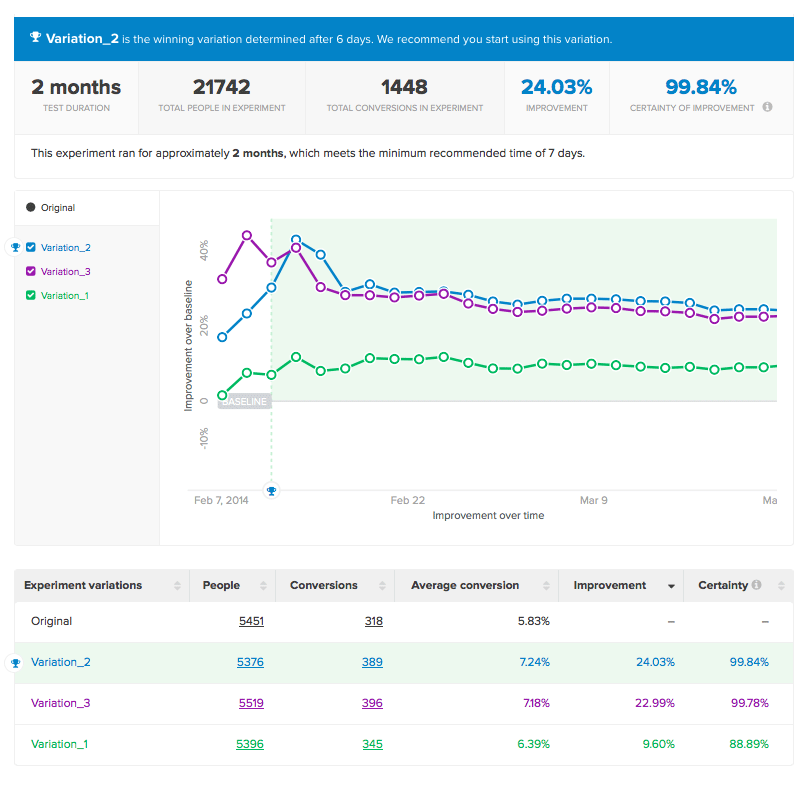
\includegraphics[max size={\textwidth},scale=0.75]{A_B}
\caption[Data získána z~A/B testování v~nástroji KissMetrics]{Data získána z~A/B testování v~nástroji KissMetrics. Zdroj: \cite{kiss-ab}}
\label{ab-fig}
\end{figure}
\newpage
\section{Shrnutí}
\par Aplikace věnující se ukládání a práci s~daty pomocí webového rozhraní se zaměřují převážně na větší podniky a obvykle nemají tolik intuitivní uživatelské rozhraní. Vylepšování dostupných aplikací není snadné a nastavení uživatelských práv je pouze v~mizivém množství dostupných aplikací. Proto se dále zaměříme na vývoj samotné aplikace, která spojí myšlenky z~aktuálních aplikací a využije open source nástroje, které umožní snadnější práci s~uživateli.
